% !TeX program = pdflatex
% =============================================================
% Public Economics -- Lecture 2
% Theoretical Tools of Public Finance
% Based on: Gruber, J. "Public Finance and Public Policy", Ch. 2
%           Stantcheva, S. "Lecture 2: Theoretical Tools for Public
%           Economics" (Harvard EC2450A, Fall 2022)
% Austrian institutional and empirical context added for WU Vienna.
% =============================================================
\documentclass[11pt,aspectratio=169]{beamer}

\usetheme{metropolis}
\usepackage[utf8]{inputenc}
\usepackage[T1]{fontenc}
\usepackage{lmodern}
\usepackage{booktabs}
\usepackage{array}
\usepackage{textcomp}
\usepackage{siunitx}
\usepackage{tikz}
\usepackage{pgfplots}
\pgfplotsset{compat=1.18}
\usepackage{pgf-pie}
\usetikzlibrary{positioning,arrows.meta,calc}

% ----------------------------------------------------------------
% Colors: WU Vienna blue as primary accent
% ----------------------------------------------------------------
\definecolor{wublue}{HTML}{003D7C}
\definecolor{wulight}{HTML}{4F8FC4}
\definecolor{wugray}{HTML}{5C6670}
\definecolor{wured}{HTML}{B0202E}
\definecolor{wugreen}{HTML}{4C8C6B}
\definecolor{wuyellow}{HTML}{D9A441}
\setbeamercolor{palette primary}{bg=wublue,fg=white}
\setbeamercolor{frametitle}{bg=wublue,fg=white}
\setbeamercolor{progress bar}{fg=wublue,bg=wulight!30}
\setbeamercolor{alerted text}{fg=wured}

\setbeamertemplate{frame footer}{Theoretical Tools of Public Finance}
\setbeamertemplate{footline}[frame number]

\title{Public Economics}
\subtitle{Lecture 2 \(\cdot\) Theoretical Tools of Public Finance}
\author{Shushanik Margaryan}
\institute{WU Vienna University of Economics and Business}
\date{Winter Term}

% Source note command for footnote-style citations on data slides
\newcommand{\srcnote}[1]{{\footnotesize\color{wugray}Source: #1}}

\begin{document}

% =============================================================
\begin{frame}
  \titlepage
\end{frame}

% =============================================================
\begin{frame}{Today's Questions}
  \begin{itemize}
    \item How do individuals choose how much to consume and how hard to work?
    \item How do firms choose how much to produce?
    \item What is the theoretical effect of raising --- or cutting --- Austria's minimum-income support (\alert{Sozialhilfe}) on economic efficiency?
  \end{itemize}
  \vspace{1em}
  \begin{block}{Based on}
    Gruber, J. \emph{Public Finance and Public Policy}, Ch.\ 2; Stantcheva, S., ``Theoretical Tools for Public Economics'' (Harvard, EC2450A).
  \end{block}
\end{frame}

\begin{frame}{Outline}
  \tableofcontents
\end{frame}

\begin{frame}{Theoretical vs.\ Empirical Tools}
  \begin{block}{Theoretical tools}
    The set of tools designed to understand the \emph{mechanics} behind economic decision making --- graphical and mathematical models of utility maximization subject to constraints.
  \end{block}
  \begin{block}{Empirical tools}
    The set of tools designed to \emph{analyze data} and answer the questions raised by theoretical analysis (the subject of Lecture 3).
  \end{block}
  \vspace{0.5em}
  \centering
  Theory tells us the \emph{direction} of an effect; data tells us its \emph{size}. We need both.
\end{frame}

% =============================================================
\section{2.1 Constrained Utility Maximization}

\begin{frame}{Utility Functions}
  \begin{block}{Utility function}
    A mathematical mapping of an individual's consumption choices into a level of well-being: $U = u(X_1, X_2, \ldots)$.
  \end{block}
  \begin{itemize}
    \item Consumers are assumed to undertake \textbf{constrained utility maximization}: maximize well-being subject to available resources.
    \item Key assumption: \textbf{non-satiation} (``more is better'') --- more of a good is always at least as good as less.
  \end{itemize}
  \vspace{0.5em}
  \centering
  \textbf{Running example:} Lena, a WU student, choosing between \emph{coffees at the Kaffeehaus} ($C$) and \emph{cinema visits} ($M$).
\end{frame}

\begin{frame}{Indifference Curves}
  \footnotesize
  \begin{columns}[T]
    \begin{column}{0.45\textwidth}
      \begin{block}{Indifference curve}
        All bundles of goods that leave an individual equally well off.
      \end{block}
      \begin{itemize}
        \item Bundle $A$: 2 coffees, 1 cinema visit
        \item Bundle $B$: 1 coffee, 2 cinema visits
        \item Bundle $C$: 2 coffees, 2 cinema visits
      \end{itemize}
      Lena is indifferent between $A$ and $B$, but strictly prefers $C$ to both (more of everything).
    \end{column}
    \begin{column}{0.55\textwidth}
      \begin{center}
      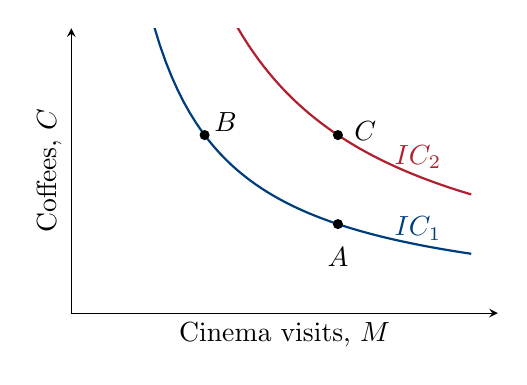
\begin{tikzpicture}
        \begin{axis}[
          width=7cm, height=5.2cm,
          xmin=0, xmax=3.2, ymin=0, ymax=3.2,
          xlabel={Cinema visits, $M$}, ylabel={Coffees, $C$},
          axis lines=left,
          ticks=none,
          ]
          \addplot[wublue, thick, domain=0.35:3, samples=60] {2/x};
          \addplot[wured, thick, domain=0.7:3, samples=60] {4/x};
          \node[wublue] at (axis cs:2.6,0.95) {$IC_1$};
          \node[wured] at (axis cs:2.6,1.75) {$IC_2$};
          \addplot[only marks, mark=*, mark size=1.6pt, black] coordinates {(1,2) (2,1) (2,2)};
          \node[anchor=west] at (axis cs:1,2.15) {$B$};
          \node[anchor=north] at (axis cs:2,0.85) {$A$};
          \node[anchor=west] at (axis cs:2.05,2.05) {$C$};
        \end{axis}
      \end{tikzpicture}
      \end{center}
    \end{column}
  \end{columns}
  Two properties (both from ``more is better''): (1) higher indifference curves are preferred; (2) indifference curves always slope downward.
\end{frame}

\begin{frame}{Marginal Utility}
  \begin{block}{Marginal utility}
    The additional utility from consuming one more unit of a good: $MU_1 = \partial u / \partial X_1$.
  \end{block}
  \begin{itemize}
    \item Example: $U = \sqrt{C \times M}$ (holding $C=2$ fixed). Moving from 0 to 1 cinema visit raises $U$ from 0 to $\sqrt{2}=1.41$; from 1 to 2 visits, $U$ rises only to $\sqrt{4}=2$ (a gain of $0.59$); from 2 to 3, the gain is only $0.45$.
    \item This is \textbf{diminishing marginal utility}: each additional unit of a good raises utility by less than the previous unit.
  \end{itemize}
\end{frame}

\begin{frame}{Aside: Does Marginal Utility Always Diminish?}
  \begin{alertblock}{Not for addictive goods}
    Becker \& Murphy (1988), ``A Rational Theory of Addiction'': today's utility from consuming a good can depend on \emph{past} consumption of it --- you build a habit.
  \end{alertblock}
  \begin{itemize}
    \item The more you have already consumed, the more you enjoy (or ``need'') consuming more --- the opposite of diminishing MU.
    \item This is a leading theoretical framework for taxing tobacco, alcohol, and sugar: if consumers systematically under-weigh future harm, corrective taxes can improve welfare beyond just correcting externalities.
  \end{itemize}
\end{frame}

\begin{frame}{Marginal Rate of Substitution}
  \begin{block}{Marginal rate of substitution (MRS)}
    The rate at which a consumer is willing to trade one good for another; equals (minus) the slope of the indifference curve: $MRS_{C,M} = MU_M / MU_C$.
  \end{block}
  \begin{itemize}
    \item For $U=\sqrt{C \times M}$: $MRS_{C,M} = C/M$.
    \item \textbf{Diminishing MRS}: as Lena has more cinema visits and fewer coffees, she is willing to give up less and less coffee for one more visit.
  \end{itemize}
  \vspace{0.3em}
  \centering
  Diminishing MRS is exactly why indifference curves are \emph{convex} (bowed toward the origin).
\end{frame}

\begin{frame}{Budget Constraints}
  \begin{block}{Budget constraint}
    All combinations of goods an individual can afford, spending her entire income: $P_C \, C + P_M \, M = Y$.
  \end{block}
  \begin{itemize}
    \item Suppose a Kaffeehaus coffee costs \texteuro{}4, a cinema ticket costs \texteuro{}8, and Lena's monthly ``fun budget'' is \texteuro{}96.
    \item Maximum coffees (0 cinema): $96/4 = 24$. Maximum cinema visits (0 coffee): $96/8 = 12$.
    \item Slope of the budget line: $-P_M/P_C = -8/4 = -2$ --- each extra cinema visit costs 2 coffees.
  \end{itemize}
\end{frame}

\begin{frame}{Constrained Choice: The Tangency Condition}
  \begin{columns}[T]
    \begin{column}{0.42\textwidth}
      \begin{itemize}
        \item Lena's optimal bundle is where her highest reachable indifference curve is \textbf{tangent} to her budget line.
        \item At that point: $MRS_{C,M} = P_M/P_C$.
        \item With $U=\sqrt{C\times M}$ and this budget: optimum is $M=6$, $C=12$ (she splits her \texteuro{}96 evenly: \texteuro{}48 on each good).
      \end{itemize}
    \end{column}
    \begin{column}{0.58\textwidth}
      \begin{center}
      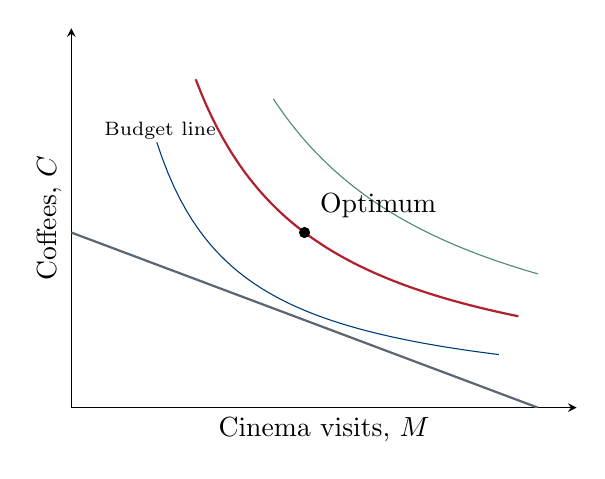
\begin{tikzpicture}
        \begin{axis}[
          width=8cm, height=6.4cm,
          xmin=0, xmax=13, ymin=0, ymax=26,
          xlabel={Cinema visits, $M$}, ylabel={Coffees, $C$},
          axis lines=left,
          ticks=none,
          ]
          \addplot[wugray, thick, domain=0:12] {96/8 - x};
          \addplot[wublue, thin, domain=2.2:11, samples=60] {40/x};
          \addplot[wured, thick, domain=3.2:11.5, samples=60] {72/x};
          \addplot[wugreen, thin, domain=5.2:12, samples=60] {110/x};
          \node[anchor=west, font=\scriptsize] at (axis cs:0.6,19) {Budget line};
          \addplot[only marks, mark=*, mark size=1.8pt, black] coordinates {(6,12)};
          \node[anchor=south west] at (axis cs:6.15,12.3) {Optimum};
        \end{axis}
      \end{tikzpicture}
      \end{center}
    \end{column}
  \end{columns}
\end{frame}

\begin{frame}{Income and Substitution Effects}
  Suppose the price of cinema tickets rises. This has two distinct effects on demand:
  \begin{block}{Substitution effect}
    Holding utility constant, a relative price rise \emph{always} causes less consumption of that good.
  \end{block}
  \begin{block}{Income effect}
    A price rise makes the consumer effectively poorer, typically reducing consumption of \emph{all} normal goods.
  \end{block}
  \vspace{0.3em}
  \centering
  For a normal good, both effects push demand in the \emph{same} direction --- toward less of the good whose price rose.
\end{frame}

\begin{frame}{Decomposing a Price Change}
  \begin{center}
  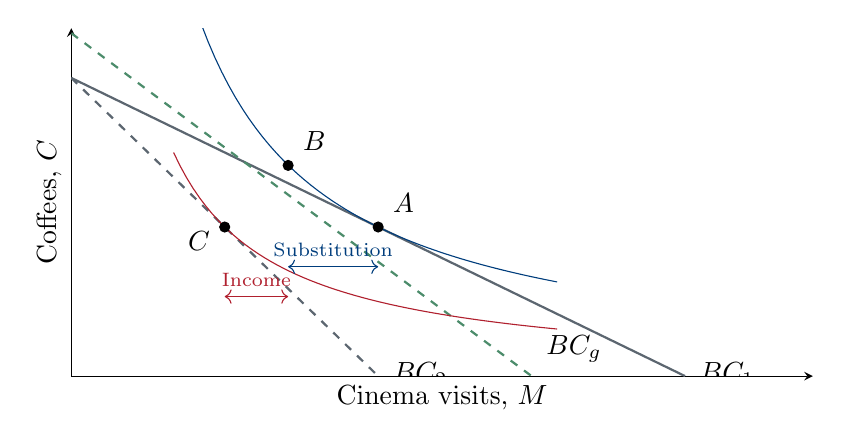
\begin{tikzpicture}
    \begin{axis}[
      width=11cm, height=6cm,
      xmin=0, xmax=14.5, ymin=0, ymax=7,
      xlabel={Cinema visits, $M$}, ylabel={Coffees, $C$},
      axis lines=left,
      ticks=none,
      ]
      \addplot[wugray, thick] coordinates {(0,6) (12,0)};
      \addplot[wugray, thick, dashed] coordinates {(0,6) (6,0)};
      \addplot[wugreen, thick, dashed] coordinates {(0,6.9) (9,0)};
      \addplot[wublue, thin, domain=1.6:9.5, samples=60] {18/x};
      \addplot[wured, thin, domain=2:9.5, samples=60] {9/x};
      \addplot[only marks, mark=*, mark size=1.8pt, black] coordinates {(6,3) (4.24,4.24) (3,3)};
      \node[anchor=south west] at (axis cs:6.1,3.1) {$A$};
      \node[anchor=south west] at (axis cs:4.34,4.34) {$B$};
      \node[anchor=north east] at (axis cs:2.9,3.1) {$C$};
      \node[anchor=west] at (axis cs:12.1,0.05) {$BC_1$};
      \node[anchor=west] at (axis cs:6.1,0.05) {$BC_2$};
      \node[anchor=west] at (axis cs:9.1,0.55) {$BC_g$};
      \draw[<->, wured] (axis cs:3,1.6) -- (axis cs:4.24,1.6) node[midway, above, font=\scriptsize]{Income};
      \draw[<->, wublue] (axis cs:4.24,2.2) -- (axis cs:6,2.2) node[midway, above, font=\scriptsize]{Substitution};
    \end{axis}
  \end{tikzpicture}
  \end{center}
  \centering \small
  Cinema price rises: $A \to C$ overall. $A \to B$ (holding utility at $IC_1$) isolates the \emph{substitution effect}; $B \to C$ isolates the \emph{income effect}.
\end{frame}

\begin{frame}{Normal vs.\ Inferior Goods}
  \begin{block}{Normal good}
    Demand \emph{increases} with income (most goods).
  \end{block}
  \begin{block}{Inferior good}
    Demand \emph{decreases} with income.
  \end{block}
  \vspace{0.5em}
  \begin{alertblock}{Austrian example}
    Public transport (\emph{Öffis}) use tends to fall as household income rises --- once people can afford a car, many drive instead. Public transport behaves like an \textbf{inferior good} over part of the income range, even though most goods are normal.
  \end{alertblock}
  \centering \small
  This is exactly why the KlimaTicket (Lecture 1) can only partly be understood through the price effect alone --- income effects and preferences over cars vs.\ transit matter too.
\end{frame}

% =============================================================
\section{2.2 Putting the Tools to Work: Sozialhilfe and Labor Supply}

\begin{frame}{Austria's Sozialhilfe (Minimum Income Support)}
  \begin{itemize}
    \item Since the 2019 \emph{Sozialhilfe-Grundsatzgesetz}, Austria's means-tested minimum income sets \textbf{maximum} rates (\emph{Höchstsätze}), not guaranteed minimums, with details varying by \emph{Land}.
    \item Maximum monthly rate for a single adult/single parent (2024): \(\approx\)\texteuro{}1{,}156. Average \emph{actual} payment to single adults: \(\approx\)\texteuro{}766/month.
    \item \S\,7 Abs.\ 6 Sozialhilfe-Grundsatzgesetz (an earnings disregard, commonly called the \emph{Wiedereinsteigerfreibetrag} in secondary sources): up to 35\% of net monthly earnings are disregarded for up to 12 months when a recipient starts working.
  \end{itemize}
  \vspace{0.3em}
  \centering
  This is Austria's own version of Gruber's TANF example --- a benefit guarantee plus a benefit-reduction rate.
  \srcnote{Sozialhilfe-Grundsatzgesetz, BGBl.\ I Nr.\ 41/2019, \S\,7 Abs.\ 6 (RIS: \texttt{ris.bka.gv.at/eli/bgbl/i/2019/41/P7}); ÖGB, ``So viel Sozialhilfe bekommt man in Österreich.''}
\end{frame}

\begin{frame}{The Consumption--Leisure Trade-off}
  \begin{itemize}
    \item Suppose Julia, a single parent, can work up to 2{,}000 hours/year at a wage of \texteuro{}10/hour, with no other income and no Sozialhilfe.
    \item Each hour of leisure ``costs'' her \texteuro{}10 in forgone wages (opportunity cost).
    \item Her budget constraint: maximum \texteuro{}20{,}000/year in consumption (0 leisure) or 2{,}000 hours of leisure (\texteuro{}0 consumption); slope $=-10$.
  \end{itemize}
\end{frame}

\begin{frame}{Adding Sozialhilfe to the Budget Constraint}
  \begin{center}
  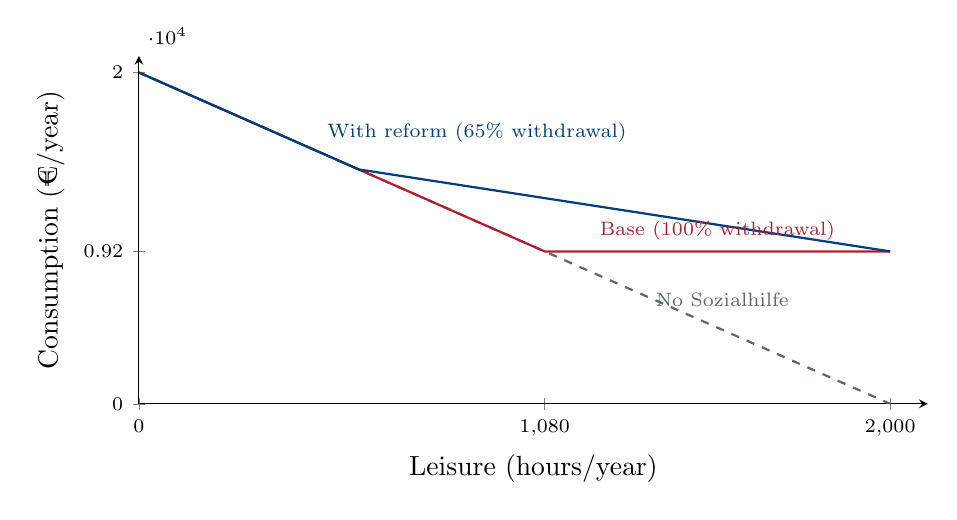
\begin{tikzpicture}
    \begin{axis}[
      width=11.6cm, height=6cm,
      xmin=0, xmax=2100, ymin=0, ymax=21000,
      xlabel={Leisure (hours/year)}, ylabel={Consumption (\texteuro/year)},
      axis lines=left,
      xtick={0,1080,2000},
      ytick={0,9200,20000},
      tick label style={font=\scriptsize},
      ]
      \addplot[wugray, thick, dashed] coordinates {(0,20000) (2000,0)};
      \addplot[wured, thick] coordinates {(0,20000) (1080,9200) (2000,9200)};
      \addplot[wublue, thick] coordinates {(0,20000) (585,14150) (2000,9200)};
      \node[anchor=west, font=\scriptsize, wugray] at (axis cs:1350,6300) {No Sozialhilfe};
      \node[anchor=south, font=\scriptsize, wured] at (axis cs:1540,9250) {Base (100\% withdrawal)};
      \node[anchor=south, font=\scriptsize, wublue] at (axis cs:900,15200) {With reform (65\% withdrawal)};
    \end{axis}
  \end{tikzpicture}
  \end{center}
  \centering \small
  Without any earnings disregard, Julia's net return to work is \texteuro{}0 until she earns her way off Sozialhilfe entirely --- a pure ``welfare trap.''
\end{frame}

\begin{frame}{The Wiedereinsteigerfreibetrag: A Real Reduction-Rate Experiment}
  \begin{itemize}
    \item \textbf{Base regime}: 100\% benefit-reduction rate. Every euro earned reduces Sozialhilfe by one euro --- net return to work is \texteuro{}0 (flat budget segment).
    \item \textbf{Reform regime}: 35\% of net earnings disregarded $\Rightarrow$ effective reduction rate \(\approx\)65\%. Net return to work rises to \texteuro{}3.50 per hour (slope $-3.5$ instead of flat).
  \end{itemize}
  \begin{alertblock}{Why this matters}
    This is \emph{exactly} the benefit-guarantee/reduction-rate logic from Gruber's TANF example --- applied to a real 2019 Austrian reform explicitly designed to soften the work disincentive.
  \end{alertblock}
\end{frame}

\begin{frame}{Predicted Effects on Labor Supply}
  \begin{itemize}
    \item Cutting the reduction rate (100\% $\to$ 65\%) makes work pay more --- a pure \textbf{substitution effect} toward less leisure (more work).
    \item But it also raises Julia's income at any given hours choice --- a competing \textbf{income effect} toward \emph{more} leisure.
    \item The net effect depends on the relative strength of the two --- and on how much Julia values leisure relative to consumption (her preferences).
  \end{itemize}
  \vspace{0.3em}
  \centering
  \alert{Theory alone cannot say whether labor supply rises or by how much --- exactly as in Gruber's Naomi/Sarah comparison.}
\end{frame}

\begin{frame}{How Large Will the Response Be?}
  \begin{itemize}
    \item The constrained-choice model tells us the \emph{direction} of well-behaved responses --- but not their \emph{magnitude}.
    \item Whether cutting Sozialhilfe's effective reduction rate actually raises single parents' labor supply, and by how much, is an empirical question.
  \end{itemize}
  \centering
  \alert{This is exactly what Lecture 3 (empirical tools) is built to answer.}
\end{frame}

% =============================================================
\section{2.3 Equilibrium and Social Welfare}

\begin{frame}{From Individual Choice to Market Demand}
  \begin{itemize}
    \item Each individual's utility maximization generates her own demand $X(P,Y)$ for a good.
    \item The \textbf{market demand curve} is the horizontal sum of all individual demands at each price.
    \item \textbf{Elasticity of demand}: $\varepsilon_D = \dfrac{\%\Delta \text{quantity demanded}}{\%\Delta \text{price}}$ --- typically negative, and typically not constant along the curve.
  \end{itemize}
\end{frame}

\begin{frame}{Supply Curves and Firms}
  \begin{itemize}
    \item Firms use a \textbf{production function} to turn inputs (labor, capital) into output, subject to \textbf{diminishing marginal productivity}.
    \item Profit maximization ($\max_Q\, [\,p\cdot Q - c(Q)\,]$) implies firms produce until \textbf{marginal cost equals price}.
    \item The marginal cost curve \emph{is} the firm's supply curve; market supply is the horizontal sum across firms.
  \end{itemize}
\end{frame}

\begin{frame}{Market Equilibrium}
  \begin{center}
  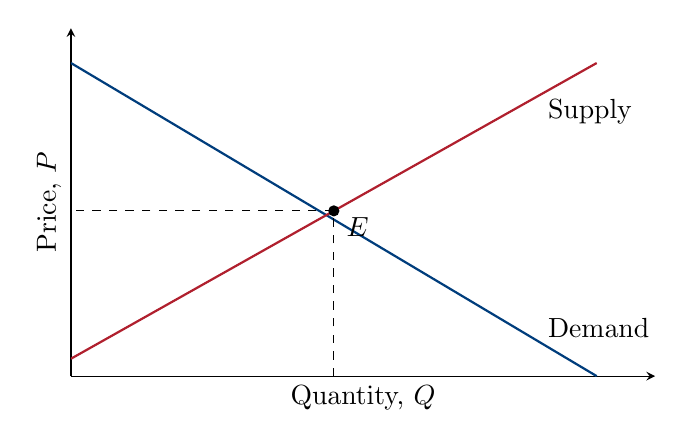
\begin{tikzpicture}
    \begin{axis}[
      width=9cm, height=6cm,
      xmin=0, xmax=10, ymin=0, ymax=10,
      xlabel={Quantity, $Q$}, ylabel={Price, $P$},
      axis lines=left, ticks=none,
      ]
      \addplot[wublue, thick] coordinates {(0,9) (9,0)};
      \addplot[wured, thick] coordinates {(0,0.5) (9,9)};
      \addplot[only marks, mark=*, mark size=1.8pt, black] coordinates {(4.5,4.75)};
      \draw[dashed] (axis cs:4.5,0) -- (axis cs:4.5,4.75) -- (axis cs:0,4.75);
      \node[anchor=west] at (axis cs:8,7.6) {Supply};
      \node[anchor=west] at (axis cs:8,1.4) {Demand};
      \node[anchor=north west] at (axis cs:4.55,4.85) {$E$};
      \node[anchor=east, font=\scriptsize] at (axis cs:0,4.75) {$P_E$};
      \node[anchor=north, font=\scriptsize] at (axis cs:4.5,0) {$Q_E$};
    \end{axis}
  \end{tikzpicture}
  \end{center}
  \centering \small
  Market equilibrium: the unique price/quantity pair at which demand equals supply, and both sides of the market are satisfied.
\end{frame}

\begin{frame}{Consumer and Producer Surplus}
  \begin{columns}[T]
    \begin{column}{0.5\textwidth}
      \begin{block}{Consumer surplus}
        The value consumers get from a good, above and beyond what they paid. Area below demand, above $P_E$.
      \end{block}
    \end{column}
    \begin{column}{0.5\textwidth}
      \begin{block}{Producer surplus}
        The profit producers earn, above and beyond their cost. Area above supply, below $P_E$.
      \end{block}
    \end{column}
  \end{columns}
  \begin{center}
  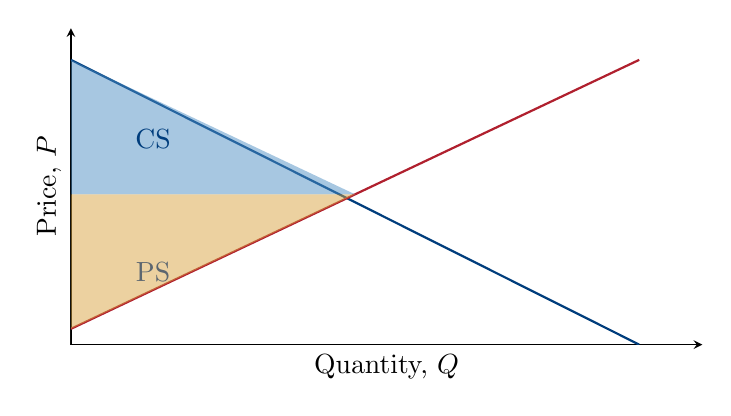
\begin{tikzpicture}
    \begin{axis}[
      width=9.6cm, height=5.6cm,
      xmin=0, xmax=10, ymin=0, ymax=10,
      xlabel={Quantity, $Q$}, ylabel={Price, $P$},
      axis lines=left, ticks=none,
      ]
      \addplot[wublue, thick] coordinates {(0,9) (9,0)};
      \addplot[wured, thick] coordinates {(0,0.5) (9,9)};
      \addplot[fill=wulight, draw=none, opacity=0.5] coordinates {(0,9) (4.5,4.75) (0,4.75)} \closedcycle;
      \addplot[fill=wuyellow, draw=none, opacity=0.5] coordinates {(0,0.5) (4.5,4.75) (0,4.75)} \closedcycle;
      \node[wublue] at (axis cs:1.3,6.5) {CS};
      \node[wugray] at (axis cs:1.3,2.3) {PS};
    \end{axis}
  \end{tikzpicture}
  \end{center}
\end{frame}

\begin{frame}{The First Fundamental Theorem of Welfare Economics}
  \begin{alertblock}{First Fundamental Theorem}
    The competitive equilibrium, where supply equals demand, maximizes total economic surplus (efficiency).
  \end{alertblock}
  \begin{itemize}
    \item Total surplus just counts \texteuro{} --- it is blind to \emph{who} gets them.
    \item Holds under: no externalities, perfect competition, perfect information, rational agents.
    \item When these assumptions fail (market failures), government intervention can potentially raise --- not just redistribute --- total surplus.
  \end{itemize}
\end{frame}

\begin{frame}{Application: Rent Regulation in Vienna}
  \footnotesize
  \begin{itemize}
    \item About \textbf{21\%} of Vienna's rented apartments are subject to the \emph{Richtwertmietzins} price ceiling (currently \texteuro{}6.74/m\textsuperscript{2}), below the market rent.
    \item A price ceiling below $P_E$ reduces the quantity landlords are willing to supply --- the classic price-ceiling case.
  \end{itemize}
  \begin{center}
  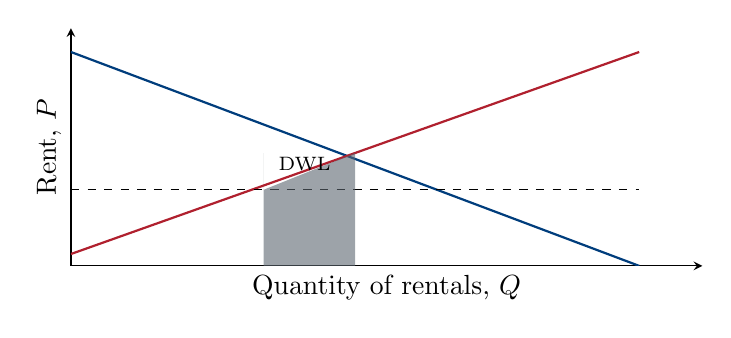
\begin{tikzpicture}
    \begin{axis}[
      width=9.6cm, height=4.6cm,
      xmin=0, xmax=10, ymin=0, ymax=10,
      xlabel={Quantity of rentals, $Q$}, ylabel={Rent, $P$},
      axis lines=left, ticks=none,
      ]
      \addplot[wublue, thick] coordinates {(0,9) (9,0)};
      \addplot[wured, thick] coordinates {(0,0.5) (9,9)};
      \addplot[dashed] coordinates {(0,3.2) (9,3.2)};
      \addplot[fill=wugray, draw=none, opacity=0.6] coordinates {(3.05,4.75) (3.05,3.2) (4.5,4.75)} \closedcycle;
      \node[anchor=east, font=\scriptsize] at (axis cs:0,3.2) {$P_R$ (ceiling)};
      \node[anchor=north, font=\scriptsize] at (axis cs:3.05,0) {$Q_R$};
      \node[font=\scriptsize] at (axis cs:3.7,4.3) {DWL};
    \end{axis}
  \end{tikzpicture}
  \end{center}
  \srcnote{Arbeiterkammer Wien, ``Richtwertmietzins''; Stadt Wien, Mietenrechner.}
\end{frame}

\begin{frame}{The Second Fundamental Theorem of Welfare Economics}
  \begin{alertblock}{Second Fundamental Theorem}
    Any Pareto-efficient allocation can be reached by (1) suitably redistributing initial endowments via \textbf{lump-sum} transfers, then (2) letting markets work freely.
  \end{alertblock}
  \centering
  If this worked in practice, there would be \emph{no conflict} between efficiency and equity.
\end{frame}

\begin{frame}{Why the Second Theorem Fails in Practice}
  \begin{itemize}
    \item Lump-sum redistribution requires the government to observe individual \emph{characteristics} (need, ability) --- not just \emph{outcomes} (income, work status).
    \item In reality, the government usually cannot tell these apart, and must base taxes/transfers on observable behavior instead.
  \end{itemize}
  \begin{alertblock}{Illustration}
    Suppose 50\% of the population is disabled and cannot work (income \texteuro{}0), 50\% can work and earn \texteuro{}100. If the government could identify disability directly, it could tax the able \texteuro{}50 \emph{regardless of whether they work}, and give \texteuro{}50 to each disabled person --- full redistribution, zero distortion.
  \end{alertblock}
  \centering \small
  But if the government cannot tell a disabled person from an able person who simply isn't working, that same \texteuro{}50 tax-and-transfer destroys the incentive to work --- redistribution now costs efficiency.
\end{frame}

\begin{frame}{Social Welfare Functions}
  \begin{block}{Social welfare function (SWF)}
    A function combining all individuals' utilities into one overall measure of social welfare.
  \end{block}
  \begin{columns}[T]
    \begin{column}{0.5\textwidth}
      \textbf{Utilitarian}
      \[SWF = U_1 + U_2 + \cdots + U_N\]
      Equal weight on every util. With diminishing marginal utility of income, favors \emph{some} redistribution from rich to poor.
    \end{column}
    \begin{column}{0.5\textwidth}
      \textbf{Rawlsian}
      \[SWF = \min(U_1, U_2, \ldots, U_N)\]
      Maximize the well-being of the \emph{worst-off} member --- generally implies \emph{more} redistribution than utilitarianism.
    \end{column}
  \end{columns}
\end{frame}

\begin{frame}{Other Social Justice Principles}
  \begin{enumerate}
    \item \textbf{Commodity egalitarianism}: society should guarantee basic needs (education, health care, retirement) as rights; beyond that, distribution doesn't matter.
    \item \textbf{Equality of opportunity}: individuals should be compensated for circumstances beyond their control (family background, ability) --- but not for the consequences of their own choices.
    \item \textbf{Just deserts}: compensation should match contribution --- taxes should track the benefits an individual receives from government (a libertarian view).
  \end{enumerate}
  \vspace{0.3em}
  \centering \small
  None of these reduce cleanly to utilitarian or Rawlsian social welfare --- real policy debates mix all three.
\end{frame}

\begin{frame}{What Do People Actually Think Is Fair?}
  \footnotesize
  Saez \& Stantcheva (2016) surveyed \(\approx\)1{,}100 US respondents with hypothetical vignettes: two people have identical pre-tax and post-tax income --- who deserves a \texteuro{}1{,}000 tax break more?
  \begin{itemize}
  \setlength{\itemsep}{2pt}
    \item \textbf{Consumption-lover vs.\ frugal person}: 74.4\% say equally deserving; only 4.1\% favor the consumption-lover (against pure utilitarianism, which would favor the higher-MU consumption-lover).
    \item \textbf{Hard-working (long hours, low wage) vs.\ leisure-lover (short hours, high wage)}: 42.7\% favor the hard-working person; only 2.9\% favor the leisure-lover.
    \item \textbf{Ranking deservingness of a benefit increase}: disabled person ranked most deserving 57.5\% of the time; a welfare recipient \emph{not} looking for work ranked \emph{least} deserving 70.8\% of the time.
  \end{itemize}
  \centering
  People reward effort and penalize perceived free-riding --- fairness judgments do not match any single textbook SWF.\\
  \srcnote{Saez, E.\ and Stantcheva, S.\ (2016), ``Generalized Social Marginal Welfare Weights for Optimal Tax Theory,'' \emph{American Economic Review}.}
\end{frame}

% =============================================================
\section{2.4 Welfare Implications of Reforming Sozialhilfe}

\begin{frame}{Efficiency: The Labor Market View}
  \begin{center}
  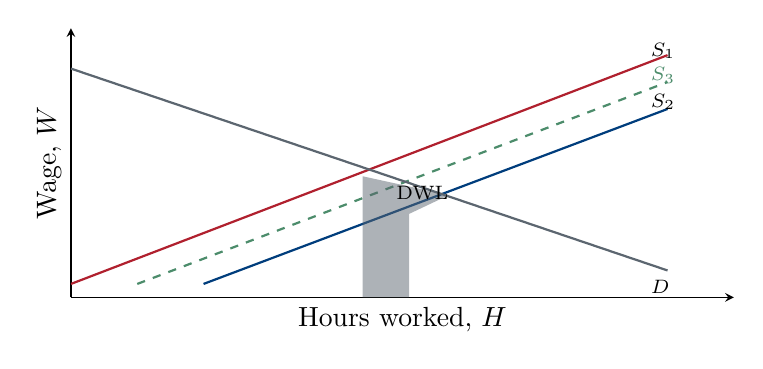
\begin{tikzpicture}
    \begin{axis}[
      width=10cm, height=5cm,
      xmin=0, xmax=10, ymin=0, ymax=10,
      xlabel={Hours worked, $H$}, ylabel={Wage, $W$},
      axis lines=left, ticks=none,
      ]
      \addplot[wured, thick] coordinates {(0,0.5) (9,9)};
      \addplot[wublue, thick] coordinates {(2,0.5) (9,7)};
      \addplot[wugreen, thick, dashed] coordinates {(1,0.5) (9,8)};
      \addplot[wugray, thick] coordinates {(0,8.5) (9,1)};
      \addplot[fill=wugray, draw=none, opacity=0.5] coordinates {(4.4,4.5) (5.7,3.8) (5.1,3.1)} \closedcycle;
      \node[anchor=south west, font=\scriptsize] at (axis cs:8.6,8.5) {$S_1$};
      \node[anchor=south west, font=\scriptsize] at (axis cs:8.6,6.6) {$S_2$};
      \node[anchor=south west, wugreen, font=\scriptsize] at (axis cs:8.6,7.6) {$S_3$};
      \node[anchor=north west, font=\scriptsize] at (axis cs:8.6,1) {$D$};
      \node[font=\scriptsize] at (axis cs:5.3,3.9) {DWL};
    \end{axis}
  \end{tikzpicture}
  \end{center}
  \centering \small
  $S_1$ no Sozialhilfe; $S_2$ base regime (100\% withdrawal); $S_3$ with the reform (65\% withdrawal); $D$ = labor demand.\\
  Sozialhilfe shifts supply left ($S_1{\to}S_2$); the reform shifts it partly back ($S_2{\to}S_3$), shrinking the deadweight loss.
\end{frame}

\begin{frame}{Equity: Single-Parent Poverty in Austria}
  \begin{itemize}
    \item \textbf{36\%} of single-parent households were at risk of poverty in 2024 --- up from just \textbf{14\%} in 2014.
    \item \textbf{43\%} were at risk of poverty \emph{or} social exclusion (the broader EU measure).
    \item Single parents spend \textbf{26\%} of income on housing, versus \textbf{12\%} for two-parent, two-child households.
  \end{itemize}
  \vspace{0.5em}
  \centering \small
  Single parents --- the population Sozialhilfe most directly supports --- are also the population for whom benefit cuts carry the largest equity cost.\\
  \srcnote{Statistik Austria, EU-SILC (2024); Sozialministerium, ``Armutsgefährdung und soziale Ausgrenzung von Ein-Eltern-Haushalten.''}
\end{frame}

\begin{frame}{The Trade-off in Practice}
  \begin{itemize}
    \item Cutting Sozialhilfe's effective reduction rate \textbf{raises efficiency} (more labor supplied, smaller deadweight loss) --- \emph{if} the substitution effect dominates.
    \item It also \textbf{worsens equity} for those unable to work more (illness, caregiving, no available jobs) --- exactly the single parents most at risk of poverty.
    \item Whichever social welfare function --- or ``just deserts'' criterion --- you find most persuasive, the trade-off does not disappear; it only shifts \emph{where} you draw the line.
  \end{itemize}
\end{frame}

% =============================================================
\section{2.5 Conclusion}

\begin{frame}{Highlights}
  \small
  \begin{itemize}
    \item Constrained utility maximization (indifference curves + budget constraint) is the workhorse model of individual choice; profit maximization plays the same role for firms.
    \item Price changes split into substitution and income effects --- both matter, and can point in different directions for the labor-leisure choice.
    \item The competitive equilibrium maximizes total surplus (1st Welfare Theorem), but says nothing about its distribution.
    \item The 2nd Welfare Theorem's promise of costless redistribution fails once government cannot observe the characteristics it would need to target --- this \emph{is} the equity--efficiency trade-off.
    \item Real people's fairness judgments (Saez--Stantcheva) don't match any single textbook social welfare function --- effort and perceived deservingness matter enormously.
    \item Theory predicts the \emph{direction} of Sozialhilfe reform's effects on labor supply, not their \emph{size} --- that requires the empirical tools of Lecture 3.
  \end{itemize}
\end{frame}

\begin{frame}{Discussion Questions for Next Time}
  \begin{enumerate}
    \item Julia's reduction rate falls from 100\% to 65\%. Sketch a case (using indifference curves) where she works \emph{less}, not more, after the reform.
    \item Is Vienna's Richtwertmietzins price ceiling more like a market failure correction or a redistribution tool? Does the 1st Welfare Theorem apply?
    \item Using the Saez--Stantcheva survey results, would you expect public support for Sozialhilfe to be higher or lower than support for old-age pensions? Why?
    \item Pick one social justice principle (commodity egalitarianism, equality of opportunity, just deserts) and use it to argue for \emph{or} against the 2019 Sozialhilfe reform.
  \end{enumerate}
\end{frame}

\begin{frame}{Sources (1/2): Textbooks \& Theory}
  \footnotesize
  \textbf{Textbooks:}
  \begin{itemize}
  \setlength{\itemsep}{2pt}
    \item Gruber, J.\ \emph{Public Finance and Public Policy}, Ch.\ 2, Worth Publishers.
    \item Stantcheva, S.\ ``Lecture 2: Theoretical Tools for Public Economics,'' Harvard EC2450A (Fall 2022).
    \item Becker, G.\ and Murphy, K.\ (1988), ``A Rational Theory of Addiction,'' \emph{Journal of Political Economy}.
    \item Rawls, J.\ \emph{A Theory of Justice} (1971, rev.\ 1999), Harvard University Press.
    \item Saez, E.\ and Stantcheva, S.\ (2016), ``Generalized Social Marginal Welfare Weights for Optimal Tax Theory,'' \emph{American Economic Review}.
  \end{itemize}
\end{frame}

\begin{frame}{Sources (2/2): Austrian Data \& Institutions}
  \footnotesize
  \begin{itemize}
  \setlength{\itemsep}{2pt}
    \item Sozialhilfe-Grundsatzgesetz, BGBl.\ I Nr.\ 41/2019, \S\,7 Abs.\ 6 (earnings disregard); Sozialministerium, ``Armutsgefährdung und soziale Ausgrenzung von Ein-Eltern-Haushalten''
    \item ÖGB, ``So viel Sozialhilfe bekommt man in Österreich''
    \item Statistik Austria, EU-SILC (2024) income and living conditions
    \item Arbeiterkammer Wien, ``Richtwertmietzins''; Stadt Wien, Mietenrechner
  \end{itemize}
\end{frame}

\begin{frame}[standout]
  Thank you!\\
  \vspace{0.5em}
  \small Questions and discussion
\end{frame}

\end{document}
